\chapter{Security}
\label{chap:security}
\emph{In this chapter, some security issues concerning virtual machines and virtualization in general are covered, which will be the basis for further research in this MA thesis.}

\section{Known non-network related security issues}

\subsection{Virusses and malware problems}

The main question we ask ourself here is the fact that if it is possible that virusses and rootkits can be transmitted from a guest VM to the host without the VM having networking capabilities? \\

As seen in the first section, virtual machines are all isolated from each other. Thus, it might seem odd that breakouks are likely to occur. However, with recent advances in technology as x86 Virtualization and I/O MMU Virtualization it turns out this is in fact possible. \\

\paragraph{I/O MMU Virtualization and DMA} With I/O MMU Virtualization, for example Intel VT-d \citep{VTD} or AMD-Vi \citep{AMDVI} it becomes possible to directly assign an I/O device such as a graphical adapter to a VM \citep{HardwareVirt4}. But it also enables Direct Memory Access (DMA). One does not have to be a security expert to see that an infected VM with Direct Memory Access can infect the memory of the host.

\clearpage

\paragraph{x86 Virtualization and rootkits} Noticable rootkits \footnote{\textbf{Rootkit:} a mostly malicious program that is designed to hide itself for detection and thus for the fact that an OS has been compromised. It is used to gain \emph{root} access (hence the name) to the compromised OS to perform, for example, eaves-dropping \citep{VMBR, Rootkit}.} are the \textbf{Blue Pill} rootkit developed by Joanna Rutkowska and the \textbf{SubVirt rootkit}, developed by Microsoft. These rootkits are two examples of VM-based rootkits (VMBR), which install an additional VMM between the host hardware and an existing operating system \citep{BluePill,LibVirt}, after which this new VMM can be used to host malicious software as illustrated in figure \ref{fig:LibVirt}.  Additionally and in contrast to usual rootkits, hypervisor-level rootkits remain undetectable, because they cannot be accessed by software \citep{BluePill,VMBR}.

One possible solution to minimize (the bluepill attack becomes impracticable) this problem from happening is to disable x86 virtualization \footnote{\textbf{x86 virtualization:} also known as hardware-assisted virtualization \citep{HardwareVirt1}, improves the performance when full virtualization is used. It adds hardware support to run VM's more efficiently. Normally, the machine code of the guest OS is translated to machine code of the host OS, by means of binary translation. With x86 virtualization - or hardware-assisted virtualization, the need for such binary translation disappears. Hardware-assisted virtualization must be supported by the CPU \citep{HardwareVirt3}. Therefore, for example Intel and AMD developed respectively Intel-VT and AMD-V for that purpose \citep{HardwareVirt2}}, despite the loss in performance. Also bear in mind that an anti-virus scanner on the host does not protect a guest VM against virusses \citep{Virus}. 
\begin{figure}[h]
	\label{fig:LibVirt}
    \centering
    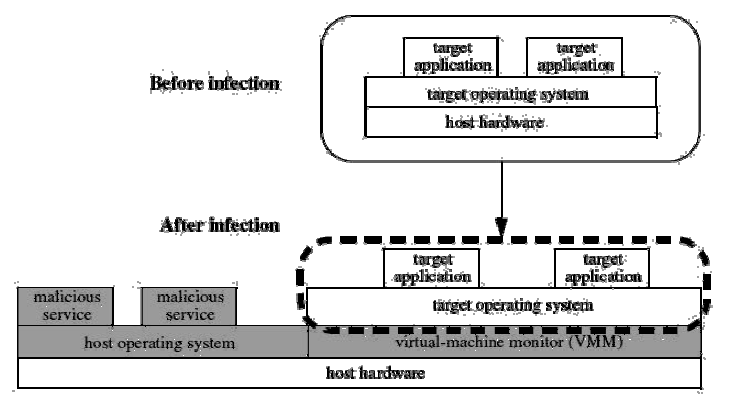
\includegraphics[width=0.7\textwidth]{VMBR.png}
    \caption[VM based rootkit]{A schematic view of a virtual machine based rootkit (VMBR). A VMM, for example Hyper-V, is installed underneath an existing OS. This means that the rootkit is now the hypervisor.}
\end{figure}

\clearpage

\section{Known network related security issues} 

When VM's are directly connected to an external network (e.g.: using Hyper-V's external network mode), then the VM is threated as any other physical machine regarding the transmission of virusses. Just a virusses spread between physical machines using files (e.g.: via mail attachments or software downloads) that are transferred through the network \citep{Virus}, the same can also happen with VM's who are connected to an external network, since when a virtual network is connected to a physical NIC, it is exposed to the same threads and security risks as that physical NIC and thus as a normal physical network\citep{Virus2}.

\section{Possible solutions}

\subsubsection{Use of firewalls}

The built-in Windows Firewall in Hyper-V does not interfere - and thus does not protect guests - with guest traffic in any way. Packets will just pass the Windows Firewall without being analyzed, because of the physical adapter bound to the virtual switch is unbound from anything that Windows Firewall has access to. \\ \\
However, extensions to the Hyper-V Virtual Switch are available that take care of these problems. A network packet filter and an intrusion detection or firewall are two out of four examples of such extensions \citep{Firewall1}.

Obviously, one can always completely isolate virtual networks from each other - and from physical networks - in order to protect the host. This can be done using VLAN's - or IP subnets - : the hypervisor (host) does not have to be on the same VLAN as the guests and thus placing it in a seperate VLAN is perfectly possible \citep{Firewall2}.


\subsubsection{Securing the guests}

As already described in the first section, virtual machines are isolated from each other, in such a way they cannot access each other's physical resources such as RAM.

However, in 2012, a security issue was found in 64 bit virtualization software running on Intel CPU's. With this vulnerability, when a system exception occured, it became possible to escape from the local guest OS into the host OS with elevated privileges, with all the consequences.

Therefore, a guest has to be secured and securing a guest is just like securing a phyiscal machine.

\subsubsection{Antimalware solution}

Attention has to be payed when installing antimalware solutions on the host OS. Either antimalware solution poses a threat to the host: most of the antimalware software dislike XML files, however, these files defines the VM's, so deleting them will cause the VM's to disappear.

This means that one has to be very careful when installing antimalware solutions and in particulary take care of exclusions.

\section{Unknown security issues}
This is what the thesis is about.